\chapter{\altGerEng{Grundlagen}{Fundamentals}}


Traditional \ac{VLC} systems utilize either positive-intrinsic-negative (PIN) \ac{PD}s or \ac{APDs} as optical receivers for high-speed photo signal reception \cite{liu2016visible}. However, both types of \ac{PD}s require external biasing power for operation \cite{wang2015design} \cite{liu2016visible}. Additionally, \ac{APDs} necessitate a high bias voltage to initiate the avalanche process within them \cite{liu2016visible}. This thesis work aims to mitigate this necessity for external biasing power. This thesis chapter, Fundamentals of the energy harvesting \ac{Li-Fi}, will be discussed.


The whole implementation of the \ac{Li-Fi} system can mainly be divided into two parts, Transmitter and Receiver \cite{mahmoud2022design}. The basic principle of a standard \ac{VLC} transmitter is to send a light signal using an LED or a LASER. A computer will be used as the source of information. The text data is sent from the PC at the transmitter to the Microprocessor via the \ac{UART} protocol \cite{mahmoud2022design}. The modulated electrical signal can be generated with Arduino or Raspberry Pi Pico. \ac{OOK} modulation can map each binary bit to a corresponding light pulse sequence. The whole transmitter system can be subdivided according to the principle of work: Information source, Information Modulation, Electrical Modulation, and finally, light signal generation.

At the receiver side, a photodetector receives the light signal from the channel medium and converts it into an Electrical current \cite{fuada2018noise}. This current can be used for both Signal Decoding and \ac{EH}, and how the signal will be separated depends on the \ac{SLIPT} method. 

After the \ac{SLIPT}, the receiver system is mainly divided into two parts: the \ac{ID} and the \ac{EH}. The \ac{ID} part of the receiver will act on the received signal that contains the data sent by the transmitter. This part of the receiver system mainly includes a \ac{TIA} as an amplifier, a Comparator, and a Demodulator. The DC part is for the Battery charge, hence \ac{EH}. This part requires a power management system containing a DC-DC boost and a Buck converter. Then it needs a supercapacitor or a lithium-ion battery for Energy storage.

\subsection{SLIPT}

\ac{SLIPT} systems have gained considerable research interest. In typical \ac{SLIPT}, the emitted optical signals are utilized simultaneously for data transmission and power transfer \cite{ding2024performance}. Figure \ref{fig:3.1} shows the basic block diagram of a \ac{SLIPT} transmitter/receiver design. \ac{SLIPT} can be achieved with three different techniques utilizing three distinct domains: i)time, ii)power, and iii)Space \cite{de2024reconfigurable}. Discussing the complete theory of the three procedures is beyond the scope of this thesis. So, this thesis will focus more on Power Splitting and Space Splitting Technique.

\begin{figure}
    \centering
    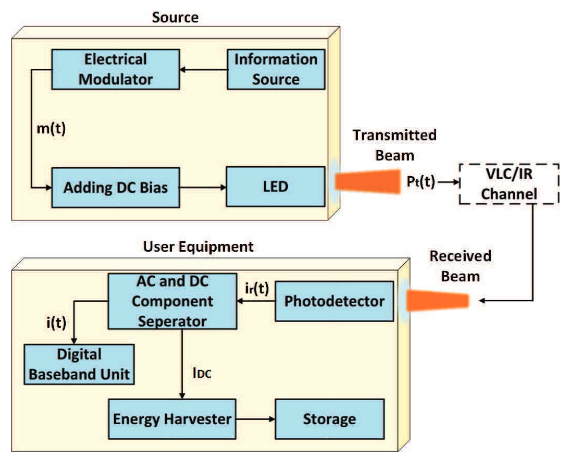
\includegraphics[width=0.75\linewidth]{fig/SLIPT transceiver design.png}
    \caption{\ac{SLIPT} transceiver design.\cite{diamantoulakis2018simultaneous}}
    \label{fig:3.1}
\end{figure}


\subsubsection{Time Switch}

Most previous work was based on the Time switch or \ac{TS} technique. \cite{de2024reconfigurable} The same receiver will switch between \ac{EH} and data receiving in two different time frames \cite{zhang2013mimo}. The problem with \ac{TS} is that its hardware implementation is complex and requires precise time control to receive synchronised data from the transmitter. 

\subsubsection{Power Splitting}

In the \ac{PS} technique, the receiver divides the power of the light signal and then uses part of it for data processing and the rest for \ac{EH} \cite{de2024reconfigurable}. Paper \cite{mahmoud2022design}, \cite{wang2015design}, and \cite{fan2017circuit} have built their model depending on the same principle.

According to \ac{PS}, the electrical signal contains AC and DC parts. The AC part is for Information decoding. AC and DC parts can be split using an electrical circuit, as in Figure \ref{fig:2.1},  and this technique is also shown in Figure \ref{fig:2.2} and \ref{fig:2.3}\cite{wang2015design}.

Using an electrical circuit to split the electrical signal after conversion offers the advantages of being less costly, highly integrated, and controllable. Add up two circuit branches after the photo device, as shown in Figure \ref{fig:2.2}, and it is possible to implement \ac{SLIPT}\cite{wang2015design}. 

\subsubsection{Space Splitting}
Conversely, the spatially separated receiver is used in the \ac{SS} technique. There are two modules, one is for the \ac{EH} and the other is for information decoding \cite{de2024reconfigurable}. Paper \cite{ma2019simultaneous} uses a spatially separated Solar panel for \ac{EH} and a \ac{PD} for information reception, shown in Figure \ref{fig:2.5}. The paper \cite{de2024reconfigurable} used spatially separated \ac{PD}s (3x3 array). For a part of the time, some \ac{PD}s are used for energy diodes, while some are used for data communication. 
Spatial splitting can have the benefits of being omnidirectional and can be implemented together with \ac{TS} and \ac{PS}\cite{de2024reconfigurable}.

\subsection{Modulation}

Data needs to be modulated with a Light signal sent by the transmitter, and this is done by an Electrical modulator shown in Figure \ref{fig:2.4} and  \ref{fig:3.1} \cite{ma2019simultaneous} \cite{diamantoulakis2018simultaneous}. Many modulation types are available for the \ac{VLC} system. \ac{OOK} is a simple, energy-efficient binary modulation scheme suitable for low-speed data transmission. Implementation of this modulation is low-cost and straightforward \cite{mahmoud2022design}\cite{6757172}, and the detection circuit is also not complex \cite{wang2022high}. It represents binary 1 as "light ON" and binary 0 as "light OFF". This modulation is not affected by the nonlinearity of the LEDs and thus improves the performance of the \ac{VLC} system. ON-OFF keying modulation can be done during Microprocessor or Arduino coding programming. In the paper \cite{mahmoud2022design}, the Arduino converts the information data into a bit stream. Design of the paper \cite{thongsa2018design} is also based on \ac{OOK}.

In paper \cite{de2024reconfigurable}, an orthogonal frequency-division multiplexing (OFDM) modulation scheme is used to achieve higher data rates exceeding 85 Mbps. It was also used in \cite{wang2015design}. Paper \cite{fan2017circuit} used Binary pulse Amplitude Modulation (PAM) because it is suitable for low-complexity demodulation circuits where energy is scarce. 


\subsection{UART}

Some encryption algorithms must be adapted to ensure a safe and secure data exchange. \cite{6757172}. A \ac{USART} is adopted in paper \cite{7420990} for better flexibility, security, and configurable communication.

The LED lamp turns on when the output bit is set to high. The data should be structured with a ten-bit pattern that includes a start bit to signify the beginning of the data byte, followed by the data byte itself, and concluding with a stop bit \cite{6757172}.

Generally, it is used in Microcontrollers and PC serial ports using the RS-232 protocol and embedded systems. While transmitting and receiving \ac{USART}s need to be at the same baud rate/ bit speed, character length, parity, and stop bits, which provides a better configuration \cite{7420990}\cite{wright_2022}.

Paper \cite{7420990} has designed a configurable communication, \ac{USART} protocol, for its \ac{VLC} system. The data exchange has been developed under the \ac{USART} unipolar Non-Return-to-Zero (NRZ) protocol. According to this paper, the circuitry design, as a result, becomes simpler and resolves power issues as it has digital pulses. 
Paper \cite{thongsa2018design} has both a transmitter and a receiver based on the \ac{UART} protocol.

\subsection{LED and LED Driver}
Generally, an LED converts the modulated electrical signal generated by an \ac{MCU} into a light signal. A White light LED is mainly used for long-distance lighting and high-speed \ac{VLC}\cite{mahmoud2022design}. It also has low power consumption and a long lifespan \cite{7420990}\cite{7292748}. A directed laser beam delivering concentrated light energy enables faster charging and higher data rates than an LED \cite{fan2017circuit}. For example, in paper \cite{fong2012integrated}, Red and Green LASER performances are compared. But using LASER has some problems, such as shadowing, power limitations, and high cost\cite{rehman2019visible}. 

An LED can have a high modulation bandwidth while also being small, low in power consumption, and sensitive. This is important for the \ac{VLC} system, where high-speed switching is necessary for transmitting information and power is limited \cite{mahmoud2022design}. 

LEDs are current-driven devices whose brightness depends on the current. So, a driver circuit is necessary for constant brightness and high-speed switching. The current can be controlled in two ways. \cite{day2004led} The first and simplest way to control the current is to use a resistor between the Power supply and the LED, depending on the desired current. However, there is a voltage drop across the resistor, hence a power dissipation, which is regarded as a waste of power.   

In contrast, a constant-current source maintains a steady current despite variations in forward voltage, resulting in consistent LED brightness. There are multiple ways to achieve this. In the paper \cite{day2004led}, the input power supply manages the voltage across a current-sense resistor instead of regulating the output voltage. This is accomplished through load disconnection, which electrically removes the LEDs from the power supply when disabled. The LED driver can also run a whole LED array if needed, for example, as shown in paper \cite{6757172}.

An LED driver circuit connects the Arduino UNO and the LED in paper \cite{bhalerao2018visible}. It is a Darlington pair consisting of two transistors suitable for rapid LED switching, shown in Figure \ref{fig:3.2}.

\begin{figure}
    \centering
    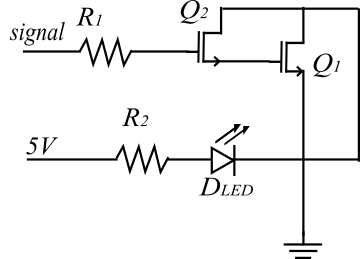
\includegraphics[width=0.5\linewidth]{fig/darlingtonpare_3.jpg}
    \caption{Darlington Pair LED circuit}
    \label{fig:3.2}
\end{figure}
One of the transistors functions as the main current-carrying transistor, while the other acts as a switching transistor that supplies the base current to drive the main transistor. This arrangement allows for a smaller base current to control a significantly larger load current since the DC gains of the two transistors are multiplied together. Thus, the combination of these two transistors can be viewed as a single transistor with an exceptionally high current gain and, as a result, a high input resistance \cite{storr_2013}.

As the goal is also \ac{EH}, some DC bias can be added to the modulated electrical signal(AC in nature). A Bias Tee circuit can correctly add DC with AC and protect the circuit from mixing before it is needed \cite{ma2019simultaneous}. This is shown in Figure \ref{fig:2.4}

\subsection{Photodetector}

Phototransistors can also detect light signals, but the \ac{PD} is more recommended because it has better linearity, dynamic range, and stability \cite{fuada2018noise}. The size of the \ac{PD} and its capacitance are small. Due to this, the response time of the \ac{PD} is much faster than that of other Photodetectors. However, the voltage generated by the \ac{PD} is small, which is insufficient for \ac{EH}. The solar panel's voltage and power is more than enough for \ac{EH}, but it has a slow response compared to \ac{PD}s. This is because the area and capacitance of a solar panel are larger \cite{fuada2018noise}.
This section will describe the basic principles of \ac{PD} and solar panels and their mode of operation.  

\subsubsection{Photodiode}

The primary output of a \ac{PD} is the current that flows through the device from cathode to anode and is approximately linearly proportional to illuminance \cite{keim_2020}. A series resistor or a current-to-voltage amplifier converts the photocurrent into a voltage for further signal processing \cite{keim_2020}.

A \ac{PD} has two operation modes, photoconductive and photovoltaic. The photovoltaic mode has several characteristics, such as a) without bias, b) non-generating dark current, c) linear, d) low noise, and e) precision instrumentation compatible. Photoconductive modes are: a) reverse bias, b) generate dark current, c) have a nonlinear characteristic, d) have significant noise, and e) are high-speed compatible. These configuration modes are illustrated in Figure \ref{fig:3.3} \cite{fuada2016trans}.

\begin{figure}
    \centering
    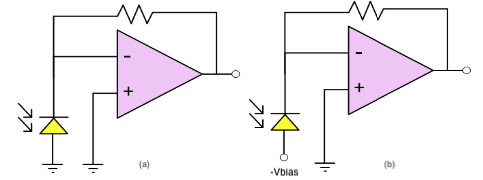
\includegraphics[width=0.75\linewidth]{fig/Photodiode Modes.png}
    \caption{\ac{PD}s mode of operation (a) Photovoltaic (b) Photoconductive.\cite{fuada2016trans}}
    \label{fig:3.3}
\end{figure}

Photoconductive mode is better for achieving higher frequencies because in this mode the depletion region is widened by reverse biasing, which makes it, in turn, faster and more sensitive to faster light signals \cite{de2024reconfigurable}.

An equivalent circuit model of an \ac{PD} is an essential analytical tool that indicates the signal that will be generated and how the \ac{PD} will interact with an amplifier circuit. Although not all \ac{PD} models are identical, they consistently include a current source, parallel capacitor, parallel resistor, series resistor, and a normal p-n junction represented by the diode symbol\cite{keim_2020} \cite{photodiodephotodiode}.

\begin{figure}
    \centering
    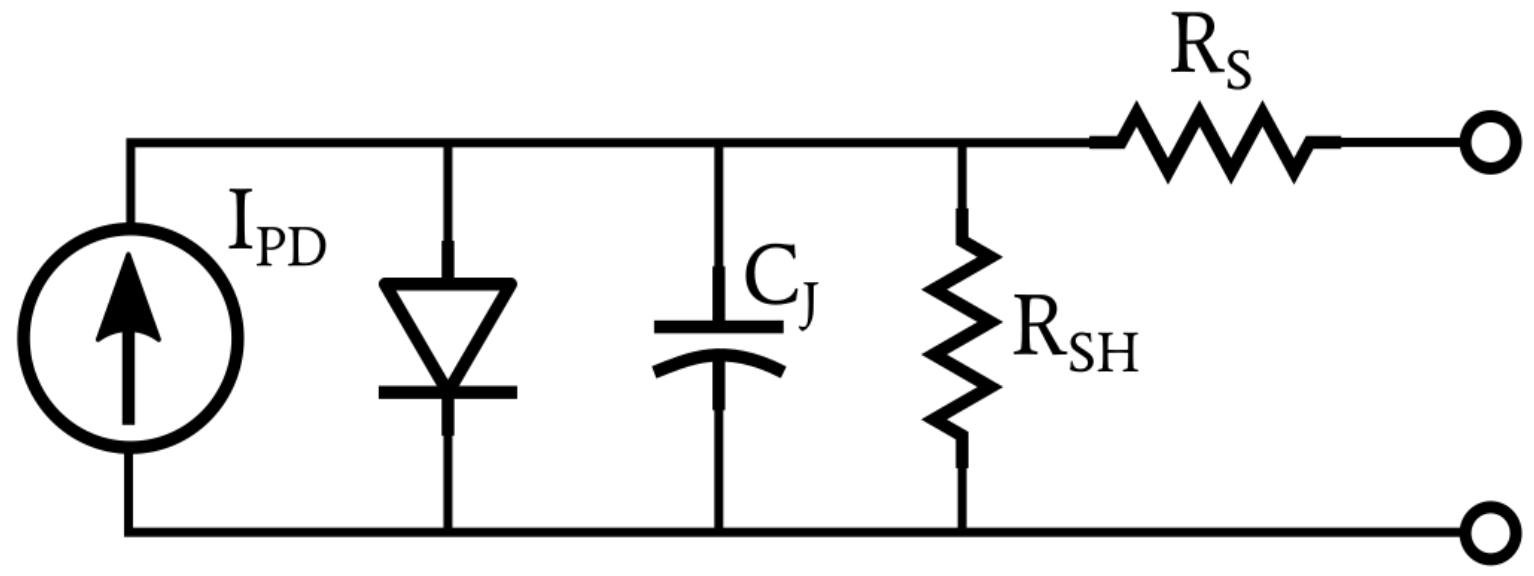
\includegraphics[width=0.75\linewidth]{fig/Photodiode equivalent circuit.png}
    \caption{\ac{PD} Equivalent circuit in Photovoltaic Mode. \cite{photodiodephotodiode}}
    \label{fig:3.4}
\end{figure}

The ideal current source (\(I_{PD}\)) represents the photocurrent and the current generated by the diode in response to incident light in Figure \ref{fig:3.4}. The parallel capacitor (\(C_{J}\)) represents the diode’s junction capacitance, the capacitance associated with the depletion region of the p-n junction. The resistor in parallel with the \ac{PD} is called the shunt resistance (\(R_{SH}\)). As with current sources, an ideal operation is achieved when \(R_{SH}\) is infinite. A \ac{PD} has contacts, wire bonds, and semiconductor material that contribute to series resistance (\(R_{S}\)). Though higher values are possible, this resistance tends to be relatively low, as in several ohms or tens of ohms\cite{keim_2020}.

A similar kind of Spice model of equivalent circuit is shown in the paper \cite{fong2012integrated} for fabricated \ac{PV} cells or \ac{PD} in PV mode shown in Figure \ref{fig:3.5}. This paper also shows that by varying a resistive load for different irradiance values, the I-V curve of the \ac{PD}s can be found, shown in Figure \ref{fig:3.6}. 
\begin{figure}
    \centering
    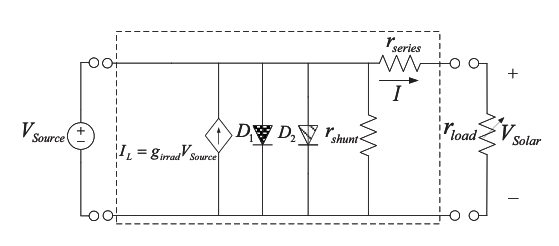
\includegraphics[width=0.75\linewidth]{fig/Generalized PV circuit.png}
    \caption{Generalized PV circuit model. \cite{fong2012integrated}}
    \label{fig:3.5}
\end{figure}

\begin{figure}
    \centering
    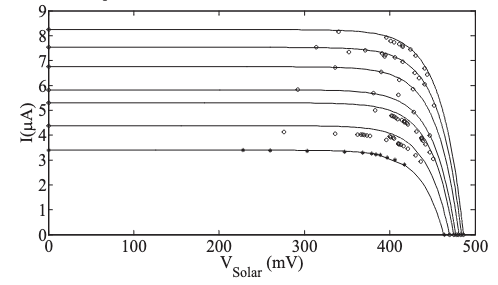
\includegraphics[width=0.5\linewidth]{fig/IV curve.png}
    \caption{IV curve of the fabricated cells}
    \label{fig:3.6}
\end{figure}

\subsubsection{Solar cell}
A solar cell is a Silicon semiconductor material divided into two doped parts: i) n-doped to provide free electrons, ii) p-doped to provide free holes. A solar cell inherently works in Photovoltaic mode. It directly generates electricity when light falls on it \cite{gallegos2015analysis}.

This current can be represented by \(I_{ph}\) and it depends on the solar irradiance \cite{4374981}\cite{wang2015design}. As a solar cell has a p-n junction, it has an inherent Diode 'D'. They are shown in the equivalent solar cell circuit, Figure \ref{fig:3.7}. 

 \begin{figure}
     \centering
     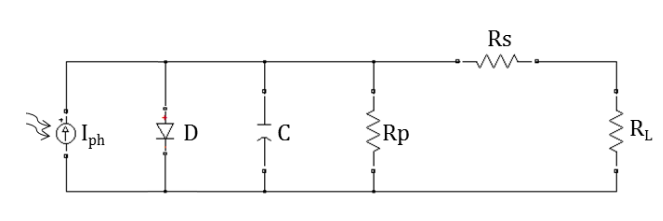
\includegraphics[width=0.75\linewidth]{fig/Electrical circuit of a solar cell.png}
     \caption{Electrical circuit of a solar cell. \cite{gallegos2015analysis}}
     \label{fig:3.7}
 \end{figure}

Here in Figure \ref{fig:3.7}, \(R_{p}\) is a parallel resistor, also known as a shunt resistor \(R_{sh}\). This represents short-circuit current losses in the cell. As short-circuit current is minimum, and current passes through \(R_{p}\) or \(R_{sh}\) should be small, and due to that, the Shunt resistance is generally high.  \(R_{s}\) is resistivity losses in the cell. This accounts for all the intersection resistance. In reality, this is not high in value \cite{gallegos2015analysis}.

Again, being a p-n junction, a depletion region is generated between the positive and negative charge regions. Due to this, a capacitance effect is produced in the Solar cell, which is represented by C in Figure \ref{fig:3.7}. This capacitance depends on the area of a solar cell. As a solar cell has a greater area than other photodetectors, it has more capacitance, and the response time increases when light falls on it\cite{gallegos2015analysis}.

Current and voltage generated by a solar cell have a non-linear relationship. The current can be represented by the equation presented in paper \cite{wang2015design} \cite{4374981} : 

\begin{equation}
\ I = I_{ph}-I_{D}-\frac{(V + IR_{s})}{R_{sh}} \
\label{eq:3.1}
\end{equation}

Here, \(I_{D}\) is Diode current and can be written as, 

\begin{equation}
\ I_{D}= I_{0}exp\left[ \frac{(V + IR_{s})}{n_{s}V_{T}}-1\right] \
\label{eq:3.2}
\end{equation}

Here, \(I_{0}\) is the reverse current of the diode, also called dark saturation current, and \(n_s \) represents the solar panel number in series connection \cite{4374981}.

Here \(V_T \) is the junction thermal voltage of the diode, which can be given by: 

\begin{equation}
\ V_{T} =\frac{AkT}{q} \
\label{eq:3.3}
\end{equation}

In this context, \( A \) represents the diode ideality factor also sometimes represented as \( \eta \), \( k \) is Boltzmann's constant, \( T \) is the temperature and \( q \) is the charge of an electron \cite{wang2015design} \cite{4374981}. The parameters \( n_s \), \( k \), \( T \), and \( q \) are known values, while the parameters \( I_{ph} \), \( I_{0} \), \( A \), \( R_{sh} \), and \( R_{s} \) are unknown variables. The overall light irradiance on the solar panel influences these unknown parameters.\cite{wang2015design}

According to the paper \cite{wang2015design}, when a solar cell is considered for communication, it is necessary to consider the AC characteristic model. Then the diode is replaced by a small-signal equivalent resistor r. A series inductor L is also necessary to represent the inductance of the wires. The complete circuit of the solar panel is already shown in Figure \ref{fig:2.2} for synchronous \ac{EH} and data
communication. Then the frequency response of the whole circuit can be given by:

\begin{equation}
\ \left[ \frac{v (\omega)}{i_{PH}(\omega)}\right]^2 = \left[ \frac{\frac{R_{LC}}{R_{s}+j\omega L+R_{LC}}*\frac{R_{C}}{\frac{1}{j\omega C_{0}}+R_{C}}}{\frac{j\omega C}{r}\frac{1}{R_{p}}\frac{1}{R_{s}+j\omega L+R_{LC}}}\right]^2 \
\label{eq:3.4}
\end{equation}

And \( R_{LC} \) is the resistance of the parallel network after the inductor L:

\begin{equation}
\ R_{LC} =  \frac{1}{\frac{1}{j \omega L_{0} + R_{L}} + \frac{1}{ \frac{1}{j \omega C_{0}} + R_{c}}} \
\label{eq:3.5}
\end{equation}

The paper \cite{wang2015design} and \cite{4374981} shows how to find these five unknown parameters:  \( R_{sh} \), and \( R_{s} \), r, C and L. \( R_{sh} \), and \( R_{s} \) can be found from I-V characteristics of the solar panel but it depends on the amount of light irradiance. Therefore, it is necessary to find out the light irradiance first and then use the I-V curve data in equation \ref{eq:3.2} \cite{wang2015design}\cite{fan2017circuit}. 

Another way is described in the paper \cite{4374981}, to use the data sheet parameters provided by the manufacturer and use the three key points of the I-V characteristics: the short-circuit point, the maximum power point, and the open-circuit point.

Parameters r, L, and C can be found from the frequency response measurement data and then put into equation \ref{eq:3.5} \cite{wang2015design}. After finding the five parameters mentioned before, it is necessary to find values of \( R_{L} \), \( L_{0} \), \( R_{c} \) and \( C_{0} \) for the proper \ac{SLIPT} circuit constructions. Methods to find them are shown in paper \cite{wang2015design} and \cite{4374981}.

In real-life applications, to have larger Power, Voltage, and current, solar cells are connected in series or parallel(depending on the application) to build a Solar array or \ac{PD} array\cite{fong2012integrated}. For example, higher voltage can be achieved by connecting \ac{PD}s in series. The paper \cite{gallegos2015analysis}, the equivalent circuit, shown in Figure \ref{fig:3.8}, and the parameter equations are given. 

\begin{figure}
    \centering
    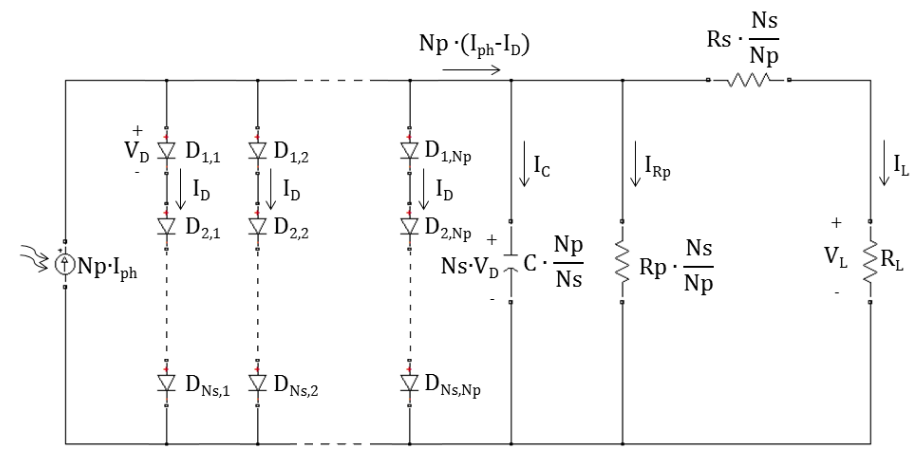
\includegraphics[width=0.75\linewidth]{fig/Electrical circuit of a solar array.png}
    \caption{Electrical circuit of a solar array. \cite{gallegos2015analysis}}
    \label{fig:3.8}
\end{figure}

Here, \(N_{p}\) is the number of solar cells connected in parallel and \(N_{s}\) is the number of solar cells connected in series. A similar kind of relationship can also be seen in paper \cite{fong2012integrated}.

The equivalent capacitance becomes, 

\begin{equation}
\ C_{eq} = C\frac{N_{p} }{N_{s}} \
\label{eq:3.6}
\end{equation}

The equivalent Shunt resistance becomes, 

\begin{equation}
\ R_{sheq} = R_{p}\frac{N_{s} }{N_{p}} \
\label{eq:3.7}
\end{equation}

The equivalent Series resistance becomes, 

\begin{equation}
\ R_{seq} = R_{s}\frac{N_{s} }{N_{p}} \
\label{eq:3.8}
\end{equation}

The current remains the same for only series-connected solar cells, and the generated voltage (open circuit voltage) is multiplied by the number of cells connected. The voltage remains the same for only parallel-connected solar cells, and the generated current is multiplied by the number of cells connected. \cite{gallegos2015analysis}. 


\subsection{Transimpedance Amplifier}

A \ac{TIA} is generally used to amplify the output of current-based sensors like \ac{PD}s, also called \ac{PD} amplifiers. In a \ac{VLC}, a \ac{PD} generates a small current proportional to the light illumination level. A high gain across the \ac{TIA} is required to overcome weak photocurrent signals and convert photocurrent output to a voltage signal\cite{fuada2016trans}.

A classical \ac{TIA}can be efficiently designed using an \ac{OPAmp} in a voltage-feedback configuration with a feedback resistor. This resistor employs negative feedback to create a low input impedance \cite{Razavi2019}. The current to be amplified is applied to the inverting input, causing the output voltage to change according to the equation:

\begin{equation}
\ V_{OUT} = -I_{IN} R_F \
\label{eq:3.9}
\end{equation}

If the open-loop gain is (\(-A_{0}\)), then he transimpedance gain is:
\begin{equation}
\ R_{T} = \frac{V_{out} }{I_{in}} = \frac{-I_{in}A_{0}R_{in} }{I_{in}} = -\frac{A_{0}}{1+A_{0}} R_F \ 
\label{eq:3.10}
\end{equation}


This topology presents a virtual ground at the input, and this minimizes the loss of signal current into the diode’s parasitic capacitance. Together with the amplifier input capacitance, this capacitance reduces the loop stability for any practicable implementation, resulting in an under-damped step response (gain peaking in the frequency response). The most common method of ensuring adequate stability is adding a small capacitance to the feedback loop, shown in Figure \ref{fig:3.9}, which provides lag compensation and can control the damping factor\cite{hayes_2002}. 

\begin{figure}
    \centering
    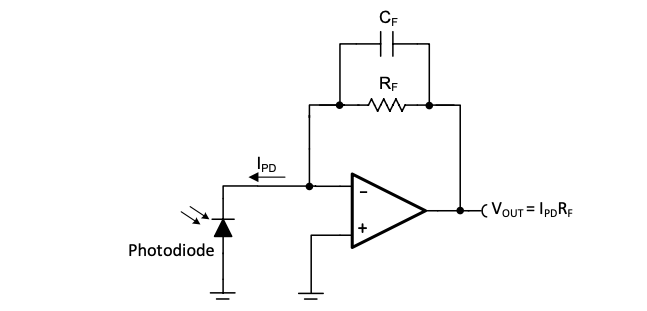
\includegraphics[width=0.75\linewidth]{fig/Connection of a photodiode to the transimpedance amplifier.png}
    \caption{Connection of a \ac{PD} to the transimpedance amplifier. \cite{caldwell1mhz}}
    \label{fig:3.9}
\end{figure}

Designing a single-supply \ac{PD} amplifier involves several important factors, such as stability and the limitations of input and output voltage ranges. Additionally, DC error sources like input bias current and input offset voltage are often overlooked, yet these can significantly affect the circuit's transient response \cite{caldwell1mhz}.

According to paper \cite{salomon}, except for the feedback resistor and capacitor, a small bias voltage must also be applied to the op amp’s non-inverting input. This prevents the output from saturating at the negative supply rail without input current.

In paper \cite{caldwell1mhz}, a resistor divider from the positive supply is used to bias the amplifier input above ground in Figure \ref{fig:3.10} to avoid saturation.

\begin{figure}
    \centering
    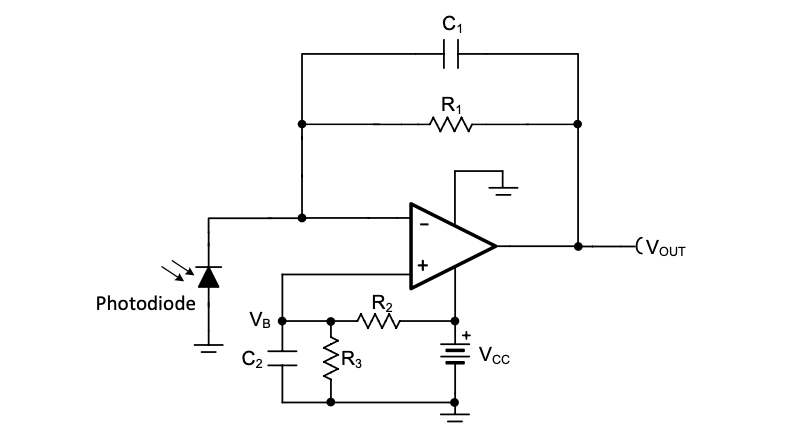
\includegraphics[width=0.75\linewidth]{fig/A bias voltage is applied to the OPAmp’s non-inverting input..png}
    \caption{A bias voltage is applied to the \ac{OPAmp}’s non-inverting input.\cite{caldwell1mhz}}
    \label{fig:3.10}
\end{figure}

Then, the output transfer function, including the bias voltage, becomes:

\begin{equation}
\ V_{OUT} = i_{PD} R_1 + V_B = i_{PD} R_1 + V_{CC} \frac{ R_3 }{R_3 + R_2} \
\label{eq:3.11}
\end{equation}

The equation gives the bias at the non-inverting input, according to Figure \ref{fig:3.10} :
\begin{equation}
\ V_{B} =  V_{CC} \frac{ R_{3} }{R_{2} + R_{3}} \
\label{eq:3.12}
\end{equation}
Then \(R_{2}\) :
\begin{equation}
\ R_{2} =   \frac{ R_{3}*(V_{CC}-V_{B}) }{V_{B}} \
\label{eq:3.13}
\end{equation}

Capacitor \(C_{2}\) is placed in parallel with resistor \(R_{3}\) to reduce the noise contribution of the resistor divider and prevent power supply noise from affecting the amplifier output. Selecting a value for \(C_{2}\)  produces a corner frequency of:
\begin{equation}
\ f_{p} = \frac{ 1 }{2 \pi C_2 (R_2||R_3)}  \
\label{eq:3.14}
\end{equation}

The value of the feedback resistor, which sets the \ac{TIA} gain \cite{fuada2018noise} \cite{salomon}, can be calculated by dividing the maximum output voltage(limited by the amplifier’s power supply) by the maximum input current:

\begin{equation}
\frac{ V_{OUT(MAX)}-V_{OUT(MIN)}}{I_{IN(MAX)}} = {R_1} \
\label{eq:3.15}
\end{equation}

The feedback capacitor with the feedback resistor builds up a pole in the frequency response of the amplifier \cite{salomon}:

\begin{equation}
\ f_{p} = \frac{ 1 }{2 \pi C_1 R_1} \
\label{eq:3.16}
\end{equation}

When the pole frequency is above this, the circuit amplification will decrease. The maximum feedback capacitor value can be calculated using the feedback resistor and the desired bandwidth \cite{salomon}:

\begin{equation}
\ C_1 \leq \frac{ 1 }{2 \pi f_{p} R_1}  \
\label{eq:3.17}
\end{equation}
The feedback capacitor needs to be kept at or below the value calculated. It ensures the circuit meets the bandwidth requirements \cite{caldwell1mhz}.

After calculating the maximum feedback capacitor value allowable to meet the design requirement for bandwidth, it is necessary to calculate the required \ac{OPAmp} gain bandwidth for the circuit to be stable \cite{caldwell1mhz}. The circuit from Figure \ref{fig:3.11} has been redrawn in Figure \ref{fig:3.10}. It shows the junction capacitance of the \ac{PD}(\(C_J)\) and the differential \((C_D)\) and common-mode \((C_{CM1}, C_{CM2})\) input capacitances of the amplifier. The bias voltage applied to the non-inverting input is considered an AC ground\cite{salomon}.

\begin{figure}
    \centering
    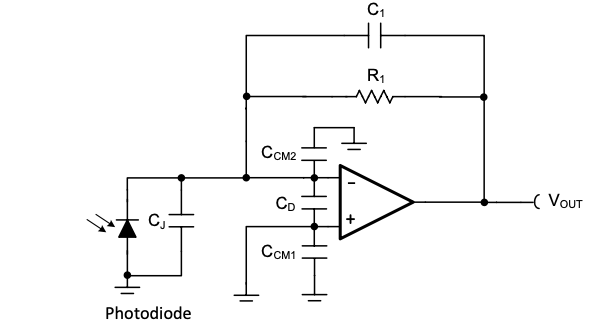
\includegraphics[width=0.75\linewidth]{fig/Transimpedance amplifier circuit showing capacitances at the inverting node.png}
    \caption{Transimpedance amplifier circuit showing capacitances at the inverting node. \cite{caldwell1mhz}}
    \label{fig:3.11}
\end{figure}

In Figure \ref{fig:3.11}, it is shown that \(C_J, C_D\), and \(C_{CM2}\) are in parallel, and the capacitance at the inverting input is:
\begin{equation}
\ C_{IN} = C_J + C_D + C_{CM2} \
\label{eq:3.18}
\end{equation}
The AC ground shorts \(C_{CM1}\) at the non-inverting input and does not contribute to the input capacitance calculation.

According to paper \cite{caldwell1mhz} for stable amplifier feedback operation the unity gain bandwidth (\(f_{GBW})\) of the \ac{OPAmp} should follow below condition:

\begin{equation}
\ f_{GBW} > \frac{  C_1 + C_{IN} }{2 \pi {C_1}^2 R_1} \
\label{eq:3.19}
\end{equation}
\(C_{IN}\)must first be determined to calculate this design's unity gain bandwidth requirement. \(C_{D}\) and \(C_{CM2}\) will be known from the data sheet of selected specific \ac{OPAmp}\cite{caldwell1mhz}.

\subsection{Comparator}

After amplifying the signal generated by a non-inverting amplifier, the output of the amplifier can be connected to a comparator for comparing the data signal\cite{thongsa2018design}. According to \cite{7420990}, a comparator can reduce noise after amplification. 

This comparison is between an input and a reference signal voltage for a non-inverting configuration. When the input signal voltage exceeds the reference signal voltage, the output signal will equal the positive level of the bias voltage. When the input signal is less than the reference voltage, the output is equal to the negative level of the bias voltage. This is called the voltage reference comparator circuit method and can be built for the receiver circuit of the \ac{VLC} system \cite{thongsa2018design} shown in Figure \ref{fig:3.12}. 
\begin{figure}
    \centering
    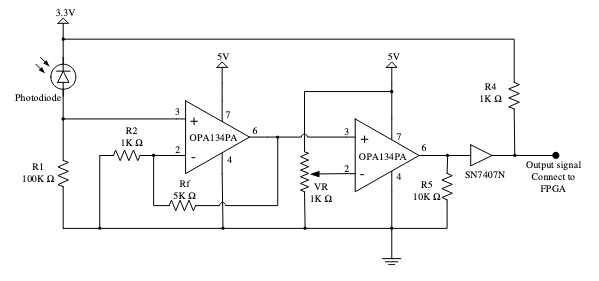
\includegraphics[width=0.75\linewidth]{fig/Comparator circuit for VLC receiver circuit.png}
    \caption{Comparator circuit for \ac{VLC} receiver circuit. \cite{thongsa2018design}}
    \label{fig:3.12}
\end{figure}

Design consideration of the comparator is provided in \cite{sboa219}, both with and without Hysteresis in the inverting configuration. The Hysteresis method is necessary where, due to noise, there are multiple transitions. Design of the comparator without Hysteresis is shown in Figure \ref{fig:3.13}. According to this design, the voltage reference is given to the non-inverting input of the \ac{OPAmp}. When one voltage divider resistor is known or fixed, the other resistor value can be determined from \ref{eq:3.20}. The voltage divider calculation is the same for inverting and non-inverting configurations, as evident by \cite{non-inverting}. 

\begin{equation}
\ V_{ref} =  V_{CC} \frac{ R_{5} }{R_{5} + R_{4}} \
\label{eq:3.20}
\end{equation}

Then \(R_{4}\) :

\begin{equation}
\ R_{4} =   \frac{ R_{5}*(V_{CC}-V_{ref}) }{V_{ref}} \
\label{eq:3.21}
\end{equation}



\begin{figure}
    \centering
    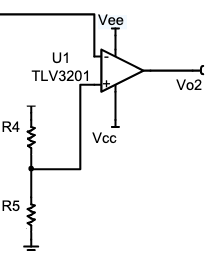
\includegraphics[width=0.25\linewidth]{fig/comparator circuit.png}
    \caption{OPAmp Comparator Circuit Design}
    \label{fig:3.13}
\end{figure}

In paper \cite{fan2017circuit}, a comparator connected with the output of the amplifier with a similar purpose is shown in Figure \ref{fig:3.15}. Except for the comparator, one can also use STM32's \ac{ADC} to sample the received signal into Digital as done in paper \cite{de2024reconfigurable}.



\begin{figure}
    \centering
    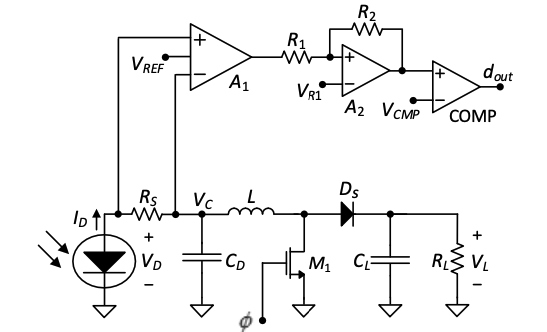
\includegraphics[width=0.5\linewidth]{fig/Schematic diagram of a DC-DC boost converter with an additional amplifica- tion circuit for data reception..png}
    \caption{Schematic diagram of a DC-DC boost converter with an additional amplification circuit for data reception. \cite{fan2017circuit}}
    \label{fig:3.15}
\end{figure}



\subsection{Storage}

According to the paper \cite{de2024reconfigurable}, harvesting power from artificial sources can not fully have the capability of self-powering all the time, and due to that, a storage must be used, preferably a supercapacitor \cite{slusbh2}. Another option would be to use a battery. However, the number of recharge cycles is limited and requires changing within two years. Considering the battery maintenance cost for complex embedded systems, supercapacitor is a more viable option, since they can be charged-discharged almost a million times and have a life span of 10 years \cite{tudose2011energy}.

Supercapacitors are an essential energy storage mechanism in self-powered systems\cite{slusbh2}. Their high energy capacities and ability to provide high power output make them ideal for ultra-low-power wireless sensor node systems. However, supercapacitors discharge significantly during periods of low-energy harvesting input. Again, this supercapacitor as a storage element can protect the system from peak currents \cite{slusbh2}.

\ac{EH} ICs are used to charge supercapacitors suffering from low efficiency during the initial charging stages until the supercapacitor reaches a nominal voltage. This causes a long wait for the supercapacitor to charge up to usable levels each time the system returns from a deep sleep state, significantly hindering the widespread adoption of supercapacitors. Also,  supercapacitors still lack energy density compared to batteries. 

Removing the battery entirely and relying solely on the supercapacitor for energy storage presents a viable solution for achieving long-lasting operation. Supercapacitors have gained significant attention recently due to their high power density, low equivalent series resistance (ESR), and minimal leakage current \cite{tudose2011energy}. 



\subsection{DC-DC Boost}

A boost converter (step-up converter) is a DC-to-DC power converter that steps up voltage (while stepping down current) from its input (supply) to its output (load) \cite{instructables_2021}. It is a class of switched-mode power supply (SMPS) containing at least two semiconductors (a diode and a transistor) and at least one energy storage element: a capacitor, inductor, or the two in combination. To reduce voltage ripple, filters made of capacitors (sometimes in combination with inductors) are typically used; only a few parts are required to make a boost converter. \cite{instructables_2021}

\begin{figure}
    \centering
    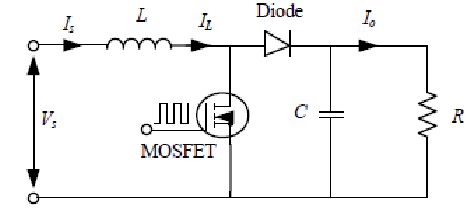
\includegraphics[width=0.5\linewidth]{fig/DC-DC boost converter circuit.png}
    \caption{DC-DC boost converter circuit.\cite{irwanto2020photovoltaic}}
    \label{fig:3.16}
\end{figure}

Due to the varying nature of ambient light, some form of DC-DC conversion and regulation is necessary to provide a stable voltage to the load. The proposed circuit in paper \cite{fan2017circuit} is based on a DC-DC boost converter, which boosts the low-voltage output of silicon photovoltaic cells. A proof-of-concept circuit was constructed and tested, as shown in Figure \ref{fig:3.16}. 



\subsection{Buck converter}

A buck converter is a step-down voltage regulator that provides non-isolated, switch-mode DC-DC conversion with simplicity and low cost \cite{ejury2013buck}. It provides the required local voltage from a higher voltage bus common to multiple converters in the system. The converter consists of one active switch controlled by an IC, a rectifier, and filter elements.

The buck converter has the filter inductor on the output side, which provides a smooth, continuous output current waveform to the load. This could be considered a qualitative benefit, but it requires special considerations for significant load transients \cite{lakshmi2014design}. A buck converter can also use pulse frequency modulation(PFM) to control the desired output voltage \cite{slusbh2}.

\begin{figure}
    \centering
    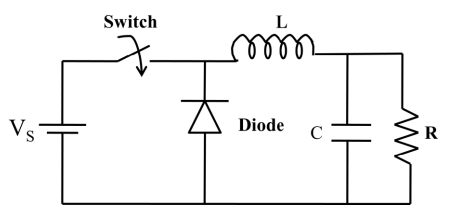
\includegraphics[width=0.5\linewidth]{fig/Schematic diagram of the buck converter..png}
    \caption{Schematic diagram of the buck converter. \cite{lakshmi2014design} }
    \label{fig:3.17}
\end{figure}
